\section{Цель работы}
Синтезировать регулятор, оптимально решающий задачу слежения за заданным задающим воздействием при заданном критерии качества.

\section{Теоретические сведения}
Рассматриваемый объект управления:
\begin{equation}
	\begin{cases}
	    \dot{x} = A x + b u, \quad x(0)\\
		y = C x
	\end{cases}
\end{equation}
где $x$~--- переменная состояния объекта, $u$~--- сигнал управления, $A$, $b$~--- постоянные и известные матрицы.

Структура синтезируемого регулятора:
\begin{equation}\label{eq_tuned_controller}
    u = K e + L_g \xi,
\end{equation}
где $K$~--- матрица коэффициентов, рассчитанная в Лабораторной работе \No2 на основе уравнения Риккати, $\xi$~--- вектор состояния модели задающего воздействия:
\begin{equation}
\begin{cases}
\dot \xi = \Gamma \xi\\
g = h \xi
\end{cases}
\end{equation}
$L_g$~--- матрица прямых связей, рассчитываемая на основе уравнения Сильвестра:
\begin{equation}
	\begin{cases}
		A M_g + b L_g = M_g \Gamma \\
		h = C M_g
	\end{cases}
\end{equation}
$e = M_g \xi - x$~--- ошибка управления.

Заданный критерий качества:
\begin{equation}\label{criteriy}
    J = \int_0^t e^T(\tau) Q e(\tau) + r (K e(\tau))^2 d\tau \ldotp
\end{equation}


\section{Исходные данные}
Варианту \textnumero2 соответствует следующий набор исходных данных:
\begin{equation}
    A =
    \begin{bmatrix}
        0 &  1 \\
        1 & -1
    \end{bmatrix}\!\!,
    \quad
    b =
    \begin{bmatrix}
        2 \\ 1
    \end{bmatrix}\!\!,
    \quad
    Q =
    \begin{bmatrix}
        1 & 0 \\
        0 & 1
    \end{bmatrix}\!\!,
    \quad
    r = 2 \ldotp
\end{equation}

Задающее воздействие:
\begin{equation}\label{g}
	g(t) = 2 \sin{8 t} + 5
\end{equation}

\vspace{0.3cm}
\section{Результаты практических действий}
\subsection{Генератор задающего воздействия}
Представим задающее воздействие~\eqref{g} в виде суммы консервативного и пропорционального звеньев.

Модель консервативного звена в пространстве состояний:
\begin{equation}\label{g1}
	\xi_1 = g,~\dot{\xi}_1 = \xi_2,~\dot{\xi}_2 = - 64\,\xi_1  
\end{equation}
где начальные условия:
\begin{equation}
	\xi_1(0) = 2,~\xi_2(0) = 0
\end{equation}

Модель пропорционального звена в пространстве состояния:
\begin{equation}\label{g2}
	\xi_3 = 5,~\dot{\xi}_3 = 0
\end{equation}
где начальные условия
\begin{equation}
	\xi_3(0) = 5
\end{equation}

Таким образом, матрица состояния генератора сигналов, векторы выхода и начальных условий, принимают вид:
\begin{equation}
	\Gamma = 
	\begin{bmatrix}
		0 & 1 & 0 \\
		-64 & 0 & 0 \\
		0 & 0 & 0
	\end{bmatrix}\!\!,~
	h = 
	\begin{bmatrix}
		1\\ 
		0\\
		1
	\end{bmatrix}\!\!,~
	\xi(0) = 
	\begin{bmatrix}
		2\\
		0\\
		5
	\end{bmatrix}
\end{equation}

\subsection{Расчет матрицы прямых связей $L_g$}
Из системы уравнений с девятью неизвестными (Вектор $L_g$ размерности $[1 \times 3]$ и матрица $M_g$ размерности $[2 \times 3]$):
\begin{equation}
	\begin{cases}
		M_g \Gamma - A M_g = b L_g \\
		h^T = C M_g
	\end{cases}
\end{equation}

Запишем девять уравнений
\begin{equation}
	\begin{cases}
		2*l_1 + 64*m_{12} - m_{21} = 0 \\
		2*l_2 - m_{11} + m_{22} = 0 \\
		2*l_3 + m_{23} = 0 \\
		l_1 + m_{11} - m_{21} + 64*m_{22} = 0 \\
		l_2 + m_{12} - m_{21} - m_{22} = 0 \\
		l_3 + m_{13} - m_{23} = 0 \\
		m_{11} - 1 = 0 \\
		m_{12} = 0 \\
		m_{13} = 0 \\
	\end{cases}
\end{equation}
Решая которые, получим элементы соответствующих матриц:
\begin{equation}
	M_g = 
	\begin{bmatrix}
		1 &          0 &          1 \\
		0.5056604 & -0.0037736 &  0.6666667
	\end{bmatrix}\!\!;
\end{equation}

\begin{equation}
	L_g = 
	\begin{bmatrix}
	  -0.2528302 &  0.5018868 & -0.3333333
	\end{bmatrix}\!\!.
\end{equation}

\subsection{Рассчитать установившееся значение $J$}
Выполним следующие операции для преобразования ошибки $e$:
\begin{gather*}
	e = M_g \xi - x,\\
	\xi = e^{\Gamma t} \xi(0) = M_\Gamma e^{\Lambda_\Gamma t} M_\Gamma^{-1}\\
	x = e^{A t} x(0) = M_F e^{\Lambda_F t} M_F^{-1}\\
	e = M_g M_\Gamma e^{\Lambda_\Gamma t} M_\Gamma^{-1} \xi(0) - M_F e^{\Lambda_F t} M_F^{-1} x(0)
\end{gather*}

Расчет критерия качества:
\begin{gather*}\textstyle
	J(t) = 	\int\limits_0^t e^T(\tau) Q e(\tau) + r e^T(\tau) K^T K e(\tau) \,d\tau =
	\\
	 \int\limits_0^t \bigl[M_g M_\Gamma e^{\Lambda_\Gamma t} M_\Gamma^{-1} \xi(0) - M_F e^{\Lambda_F t} M_F^{-1} x(0) \bigr]^T Q \bigl[ M_g M_\Gamma e^{\Lambda_\Gamma t} M_\Gamma^{-1} \xi(0) - M_F e^{\Lambda_F t} M_F^{-1} x(0) \bigr] \,d\tau + {}
	\\
	{} + \int\limits_0^t r \bigl[ M_g M_\Gamma e^{\Lambda_\Gamma t} M_\Gamma^{-1} \xi(0) \bigl]^T  K^T K  \bigl[ M_g M_\Gamma e^{\Lambda_\Gamma t} M_\Gamma^{-1} \xi(0) \bigl] \,d\tau = {}
	\\
	{} = \bigl[ M_\Gamma^{-1} \xi(0) \bigl]^T \Biggl( \int\limits_0^t e^{\Lambda_\Gamma t} R_1 e^{\Lambda_\Gamma t} \,d\tau \Biggl) M_\Gamma^{-1} \xi(0)  + {}
	{} + \bigl[ M_F^{-1} x(0) \bigl]^T \Biggl( \int\limits_0^t e^{\Lambda_F t} R_2 e^{\Lambda_F t} \,d\tau \Biggl) M_F^{-1} x(0)  + {}
	\\
	{} + \bigl[ M_\Gamma^{-1} \xi(0) \bigl]^T \Biggl( \int\limits_0^t e^{\Lambda_\Gamma t} R_3 e^{\Lambda_F t} \,d\tau \Biggl) M_F^{-1} x(0)  + {}
	{} + \bigl[ M_F^{-1} x(0) \bigl]^T \Biggl( \int\limits_0^t e^{\Lambda_F t} R_4 e^{\Lambda_\Gamma t} \,d\tau \Biggl) M_\Gamma^{-1} \xi(0)  = {}
	\\
	{} = \bigl[ M_\Gamma^{-1} \xi(0) \bigr]^T \left(  \left. \left( e^{\Lambda_\Gamma \tau} \Lambda_\Gamma^{-1} e^{\Lambda_\Gamma \tau} - \Lambda_\Gamma^{-1} \frac{(e^{\Lambda_\Gamma \tau})^2}{2} \right)\right|^t_0 \right) R_1\, M_\Gamma^{-1} \xi(0) + {}
	\\
	{} = \bigl[ M_F^{-1} x(0) \bigr]^T \left(  \left. \left( e^{\Lambda_F \tau} \Lambda_F^{-1} e^{\Lambda_F \tau} - \Lambda_F^{-1} \frac{(e^{\Lambda_F \tau})^2}{2} \right)\right|^t_0 \right) R_2\, M_F^{-1} x(0) + {}
	\\
	{} + \bigl[ M_\Gamma^{-1} \xi(0) \bigl]^T \Biggl( \cdots \Biggl) M_F^{-1} x(0)  + {}
	\\
	{} + \bigl[ M_F^{-1} x(0) \bigl]^T \Biggl( \cdots \Biggl) M_\Gamma^{-1} \xi(0)
\end{gather*}
\begin{ESKDexplanation}
	\item[где ] $F = A - b K$ размерности $[2 \times 2]$;
	\item $\Gamma$ размерности $[3 \times 3]$;
	\item $M_F$~--- матрица собственных векторов матрицы~$F$;
	\item $\Lambda_F$~--- диагональная каноническая форма матрицы~$F$;
	\item $M_\Gamma$~--- матрица собственных векторов матрицы~$\Gamma$;
	\item $\Lambda_F$~--- диагональная каноническая форма матрицы~$\Gamma$;	
	\item $R_1 = \bigl[ M_g M_\Gamma \bigl]^T ( Q + r K^T K ) M_g M_\Gamma$ размерности $[3 \times 3]$;
	\item $R_2 = M_F^T ( Q + r K^T K ) M_F$  размерности $[2 \times 2]$;
	\item $R_3 = \bigl[ M_g M_\Gamma \bigl]^T ( Q + r K^T K ) M_F$ размерности $[3 \times 2]$;
	\item $R_4 = M_F^T ( Q + r K^T K ) M_g M_\Gamma$ размерности $[2 \times 3]$.
\end{ESKDexplanation}

Исходная матрица коэффициентов обратных связей:
\begin{equation}
    K = \begin{bmatrix}0.8877665&0.5376567\cr \end{bmatrix}\!\!\ldotp
\end{equation}
Критерий качества:
\begin{equation}
	J(4.5) = 51.215047
\end{equation}

При увеличении компонентов матрицы~$K$ на 20\%:
\begin{equation}
    K = \begin{bmatrix}1.0653198&0.6451880\cr \end{bmatrix}\!\!,
\end{equation}
Критерий качества:
\begin{equation}
	J(4.5) = 52.304977
\end{equation}


Графики переходных процессов в рассматриваемой системе при двух выше приведенных версиях матрицы~$K$ показаны на рисунке~\ref{img_graphs},
а использованная для их получения схема моделирования~--- на рисунке~\ref{img_modeling_scheme}.
\begin{figure}[h!]
	\centering
	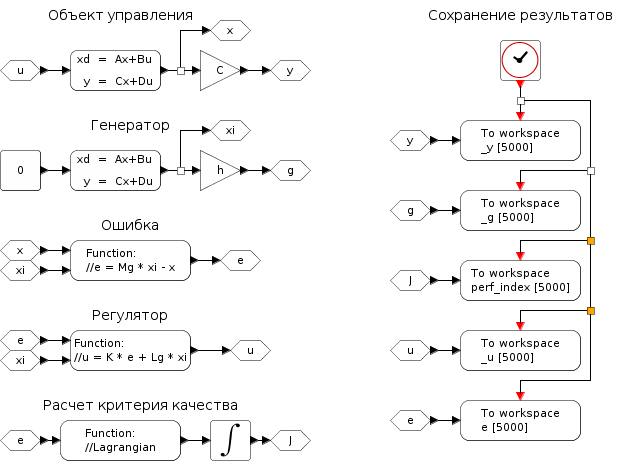
\includegraphics[width=0.8\textwidth]{modeling_scheme.png}
	\vspace{0.5cm}
	\caption{Схема моделирования рассматриваемой системы управления.}
	\label{img_modeling_scheme}
\end{figure}
\begin{figure}[h!]
    \centering
    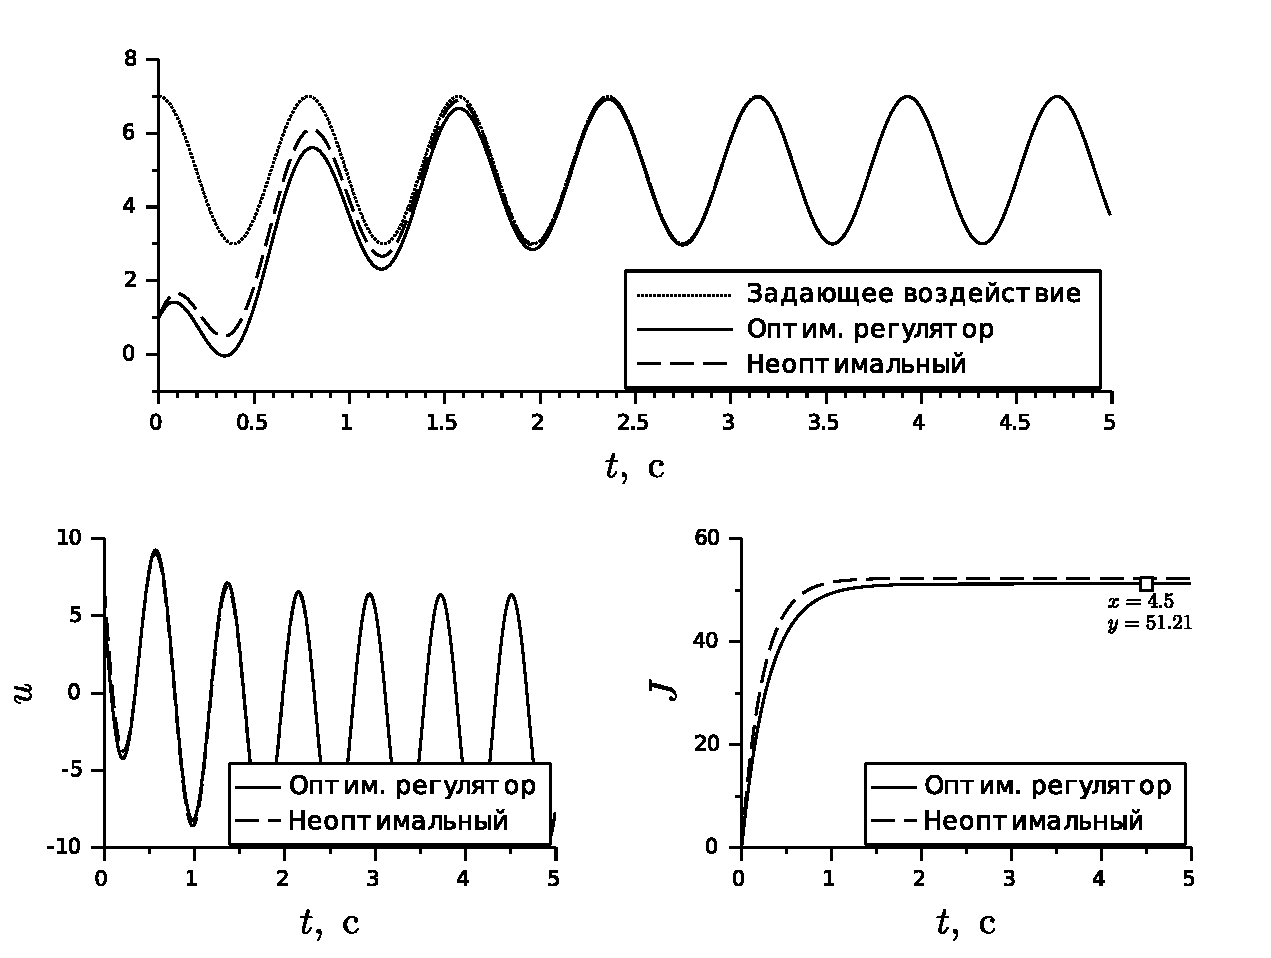
\includegraphics[width=\textwidth]{graphs.pdf}
    \vspace{0cm}
    \caption{Графики переходных процессов при оптимальном и неоптимальном регуляторах.}
    \label{img_graphs}
\end{figure}

\newpage

\section{Выводы по работе}
В~результате проделанной работы для заданного объекта управления был рассчитан регулятор, оптимальным образом решающий задачу слежения за задающим воздействием~$g$~\eqref{g} с точки зрения минимизации значения критерия качества~$J$~\eqref{criteriy}. Последнее было проверено отклонением коэффициентов регулятора от их рассчитанных значений~--- как и следовало ожидать, установившееся значение критерия качества в таком случае оказалось больше, чем при оптимальном~$K$.
